\documentclass[conference]{IEEEtran}
\IEEEoverridecommandlockouts
% The preceding line is only needed to identify funding in the first footnote. If that is unneeded, please comment it out.
\usepackage{cite}
\usepackage{amsmath,amssymb,amsfonts}
\usepackage{algorithmic}
\usepackage{graphicx}
\usepackage{textcomp}
\usepackage{xcolor}
\def\BibTeX{{\rm B\kern-.05em{\sc i\kern-.025em b}\kern-.08em
    T\kern-.1667em\lower.7ex\hbox{E}\kern-.125emX}}
\begin{document}

\title{Deep Neural Nets-based Value Predicting Mechanism and Autoscaling Approach using Deep Reinforcement Learning for Microservice Workloads in Cloud Environments\\
}

\author{\IEEEauthorblockN{Anusha S, Darshan V, G Sriram Sharath, Christina Joseph, K Chandrasekaran}
\IEEEauthorblockA{\textit{Department of Computer Science and Engineering} \\
\textit{NITK Surathkal}\\
Mangalore, Karnataka, India 575025}
}

\maketitle

\begin{abstract}
The field of cloud computing is changing in field of computer science. Software companies are using cloud services to deploy their applications. As a result, a lot of interest has been shown by researchers in this field. An important challenge faced in this field is the question of how and when to scale the use of hardware and virtual machine resources. As cloud services are costly, making efficient use of them is necessary to prevent wastage of resources and which will help companies in preserving there business. In this paper, we present a parameter value predictor using LSTMs and RNNs, both of then different predictive mechanisms using neural networks and finding out which is more effective. Previously, approaches like different processing, mathematical models were used to scale microservices. Those approaches were not optimal as they are not good at predicting loads and hard to manage. So, we use Reinforcement Learning, namely Double Deep Q-Networks Algorithm, as this approach automatically monitors the parameters which are essential for scaling and triggers the effect (action) onsite immediately. It also balances the acts of exploiting the environment and exploring the environment, using the computing resources and computing cost-effectively.
\end{abstract}

\begin{IEEEkeywords}
autoscaling, reinforcement learning, double DQN,Average Memory Utilization SLA
\end{IEEEkeywords}

\section{Introduction}
Generally, application deployment used to be done in the monolithic architecture approach. These applications usually contain a single directory. Multiple instances of the application can be run when the number of clients increases and the load needs to be balanced. To overcome the numerous limitations such as overloaded containers and IDEs, dynamic scaling not being possible, a new software architecture called microservice architecture was introduced which divides the application into atomic modules. It scales these modules instead of the entire application i.e, new instances of the modules are created when scaling is done instead of creating new instances of the application. This model provides improved fault tolerance and improved maintainability among other benefits. \\

In microservice architectures, cloud service providers face the challenge of ensuring that Service Level Agreement violations do not take place. Service Level Agreements usually specify the performance expected from the computing infrastructure and failure to adhere to it will lead to monetary penalties. At the same time, cloud service providers also have physical and financial constraints to scale up or down. Thus, ensuring that the hardware resources, power, etc. offered by the Cloud providers are used at an optimal level is a tough question to answer. \\


Predicting when to scale in a model is most important their are different prediction available among those we chosen Long short-term memory (LSTM) which is an artificial recurrent neural network (RNN) architecture used in the field of deep learning. In an LSTM network, as opposed to a typical feed forward neural network, there are feedback connections. Along with processing data with individual points, images for example, it can also process data sequences, like speech and video. A standard LSTM entity has the following components: a memory component called cell, and three gates for overseeing the information flow, called input, output, and forget. \\

An RNN formed using LSTM entities can undergo supervised training on a predetermines training data, employing an optimization algorithm such as gradient descent, along with back propagation to calculate the loss gradients. Values of errors are sent back from  output layer, and it is saved in the cell of the LSTM entity. Such a mechanism enables continuous learning from the errors.\\

Reinforcement Learning is a class of machine learning that does not require labeled datasets or any supervision. The model has zero knowledge about the environment and it makes its own decisions based on trial and error approach and develops policies that will yield our rewards and punishments based on the action done for a particular state. This is done for n episodes till we get an accurate model. Generally, training in reinforcement learning is a very lengthy process as it takes a long time for values to converge to a point and it consumes a lot of memory for storing action-state pairs.This can be solved by Deep Reinforcement Learning where we use Q-value function and convolutional neural networks to predict the future rewards and actions to be taken at a particular state so that we get maximum rewards. This approach minimizes memory wastage when we deal with a large number of state-action pairs. In this paper, we have described the working of an LSTM based value predictor which can be given as input for a DDQN to take autoscaling decisions based on the Average memory Utilization. We try to design and develop an autoscaling policy for microservices using Deep Reinforcement Learning. 

\\

\section{Autoscaling Algorithms}

Scaling is the ability of cloud computing resources to handle increasing or decreasing demands in a flexible and graceful manner. Scaling is classified into horizontal and vertical scaling based on how computing resources are distributed in the infrastructure. In horizontal scaling, we add more machines to a pool of machines and in vertical scaling, we add more power/resources to an existing machine. In our project, we will be using the Horizontal Pod Autoscaler along with a Double DQN service. Horizontal Pod Autoscaler modifies the number of replicas based on the current memory being used. If the memory utilization increases, HPA will create new instances, for which there may or may not be enough space in the cluster. If there are not enough resources, Cluster Autoscaler will try to bring up some nodes, so that the HPA-created pods have a place to run. If the load decreases, HPA will stop some of the replicas. As a result, some nodes may become underutilized or completely empty, and then the Cluster Autoscaler will terminate such unneeded nodes.
\\

Based on when scaling decisions are taken, scaling is divided into reactive scaling and proactive scaling and hybrid scaling. In reactive scaling, resources are scaled based on loads that have already appeared. In proactive scaling, resources are scaled based on loads that are expected to appear in the future. In the hybrid type, a combination of proactive and reactive scaling is used. For example, containers or virtual machines may be scaled using a reactive approach but individual pods inside the containers are scaled using a proactive approach. In our project, we use the hybrid scaling approach. We use an LSTM model to predict metric values, which will be sent to the Double DQN module to take scaling decisions.  
\\

Generally, parameters like CPU usage, memory usage, requests served per unit time are the parameters used by most researchers to make scaling decisions as these are the parameters which are directly obtained from the machine and so, give us a better picture about the state of the machines which we are trying to scale. Metrics like packet rate, bandwidth, average end to end delay are obtained from the machines as well, but they tell us more about the state of the network than about the state of the machine. 
\\

\section{Reinforcement Learning}


% \begin{equation}
% a+b=\gamma\label{eq}
% \end{equation}

Reinforcement Learning is a class of machine learning that does not require labeled datasets or any supervision. Here, an agent learns to solve a problem using the trial and error method. For every action the agent performs in the environment, there is either a reward or a penalty. The goal of the agent will be to maximize the value of the rewards as it learns through each and every iteration. Here, it is the programmer who sets the rules i.e, the rewards and penalties for a given problem. Another important feature of reinforcement learning is that the agent does not spend all its time on maximizing the rewards. There are times when it will settle for a smaller reward in the present so that it may get a bigger reward in the future. This act of settling for a lower reward at the present at the possibility of getting a bigger reward in the future is called exploration. On the other hand, preferring to stay with the option of getting a bigger score is called exploitation. Reinforcement learning systems need to balance both these tasks. In general, a bulk of the time, about 80\%-90\% is spent on exploitation and the remaining time is spent on exploration. This strategy is called the epsilon-greedy strategy. 
\\
Usually, problems solved using Q-Learning can be formalized as a Markov Decision Process problem. And Markov Decision Processes include the following: a finite set of states, a set of actions available for each state, transitions between states, rewards associated with each transition, a discount factor between 0 and 1 that quantifies the difference in importance between immediate rewards and future rewards. 
\\
Q-learning is a strategy that decides what action to take on the basis of a variable of self-value that defines the value of being in a given state or doing any action at that state. We have a Q feature that takes one state and one action as input and returns the predicted reward (and all future actions) of that action. Q gives the same (arbitrary) fixed value until we explore the setting. But then, when we further analyze the setting, Q gives us a good estimation of the worth of a specific action at a given state. The Q function is updated as we run more and more iterations. This is a formula that demonstrates how to solve a problem using Q-Learning.
\\

\begin{figure}[htbp]
\centerline{\includegraphics[width=8cm,height=3cm,keepaspectratio]{equation.png}}
\caption{Equation 1}
\end{figure}

\\
These are the variables which are used in the given equation: 
\\
Alpha: This is the learning rate, which specifies how aggressive our algorithm should be when it wishes to update score values. 
\\
Reward: It is the particular reward obtained for taking up a particular action at a particular state. 
\\
Gamma: It is the discount factor parameter that quantifies the difference in importance between immediate rewards exploitation and the remaining time is spent on exploration. This strategy is called the epsilon-greedy strategy. 
\\
However, if we only use Q-learning, it has its disadvantages concerning memory and time to make decisions, so Deep Reinforcement learning was introduced to overcome this disadvantage. Using this, we can generalize the Q-function values and rewards for the future, unlike normal Q-learning, where we need to store each every Q-function value and search for the highest Q-value from the table, which is time taking and long. So in deep RL, we have a network layer introduced where we create the network to predict the value of the upcoming Q-function and give the reward according to the q value predicted, which reduces our work.
\\
Even if we use deep Q-networks to predict the best Q-value from the Q-function, it overestimates the value as it always tries to make greedy decisions. It creates what is called maximization bias in the learning part with the overestimation causing many problems such as creating as giving importance to unnecessary decisions in policy, which will reduce the efficiency of our network. So in order to overcome this problem, a different version of DQN was introduced, which was called Double DQN. It was able to solve the problem as it used two networks, namely a Deep Q network and Target  Q network, which help us to check the decisions made by the network using the target network and add that decision to the policy. This will help us to reduce the overestimations and get better Q-values. As a result, we are using this approach for our implementation, where we take a set of actions and states for scaling based on the Q-value generated by the double DQN to scale out the application or not in the cloud platform, which efficient. 
\\

\section*{Related Work}

Yenel et al. propose a model that uses proactive scheduling, and the scaling is done by iterating through a set of states to be achieved among a given set of states, an idea which is used in our project. Podolskiy et al. propose a predictive scaling model is used, but requests per second are used as a parameter for making scaling decisions[13]. The graph-based model of the microservice application is used to balance the application capacity statically. The schedule of future scaling actions is generated according to one of the following policies: Naive, best resource pair, only-delta-load policy. However, the downside of this paper is that it is limited to microservice web applications with a homogeneous workload. Models employed are limited by the capacity of the application expressed in terms of RPS. \\ \\

Kwan et al. propose a reactive scaling model can be used with CPU utilization the metric for scaling[14]. If the resource allocation is higher than the usage and signals to the algorithm that there are unused CPU resources for this microservice. For every such microservice, downward vertical scaling (i.e., resource reclamation) is attempted on each of their replicas to move the instance towards the target utilization. If an instance has been vertically scaled downwards and its allocated resources drop below a minimum threshold, it is removed entirely. The opposite is done for upward scaling[15]. This algorithm is unable to handle memory-bound loads and crash. Gias et al. propose a model where the length of message queues is used as a measure for scaling. Scaling decisions are taken by solving multiple LQN models. To generate these models, queueing theory is used. Baeur et al. propose a model where predictive scaling is used coupled with a reactive fallback. To obtain good forecasts with a model of the seasonal pattern, the availability of two days of historical data is required. This proposed model requires an external monitoring component that collects the required values. The main disadvantage is that each service instance is deployed on homogeneous resources[16]. Song et al. propose a hidden layer of RNN is replaced with the LSTM block learning long-term dependencies for predicting metric values for scaling[17]. Kumar et al. propose a model where one can predict the metric values using a three-layered neural network. It uses self-adaptive differential evolution for training neurons in the neural network. However, this is a costly approach compared to the one mentioned in [17], so we have decided to go with LSTM for our project. \\ \\

Li et al. propose a paper where reactive scaling is used, and the average end to end delay is used as the metric for scaling. If the average end to end latency is more than the maximum agreed upon in the SLA, scaling up is performed. The problem with this approach is that end to end delay is affected by external factors relating to networking conditions, including interference, channel errors and congestion[19]. \\ \\

Li et al. propose a mechanism which tries to use multiple metrics. Proactive scaling is done using packet rate, link bandwidth and the number of cores as the metric. It uses a linear programming model with randomized rounding to efficiently and proactively obtain a near-optimal solution [20]. Hyun Woo Kim et al. propose a mechanism which uses reactive scaling; the storage size used by the user is analyzed based on the time per month to identify expected fixed storage size. Performance information is analyzed based on clustered desktop resources [21]. Performance information is analyzed separately for dynamic performance factors (idle CPU performance, residual memory, and storage sizes) and static performance factors (performance of the underlying CPU installed in the desktop, maximum sizes of the memory and storage). Another paper proposes using a complicated context switching method, along with a hybrid mechanism and a combination of horizontal-vertical scaling[22]. \\ \\

Gu et al. studied application needs and their performance requirement (virtual queueing system) is used as a metric for scaling[23]. A shadow routing algorithm maintains virtual queues and a greedy Primal-Dual (GPD) applied to the virtual system. In [24], hybrid scale-up and horizontal scale-down are used. Based on the queueing model, prediction of the arrival time of each customer is made, then the calculation of the minimum amount of resources that meet the resource needs is done. Compared with the traditional method that fixedly deploys resources by the peak load, this method can effectively improve the resource utilization and guarantee the quality of service. \\ \\

Rossi et al. propose RL based Solutions for Container Deployment and adaptation in the real-time environments of cloud services[5]. Generally, there are two types of scalings Horizontal and Vertical for the deployment of containers; most of them use Horizontal scaling. Fabiana Rossi, the author, combines both of these scaling methods and uses RL to apply the scaling or not under varying workload conditions. RL is model-free, and because of that, it takes a longer time to build a good model as it does not have a priori knowledge about the environment. So author Uses a Model-based approach to overcome this disadvantage so that our agent can adapt to the environment faster and better resource usage whenever there is a change in the environment. Validation of his work was done by implementing his approach in Docker Swarm, which adapts to the environment accordingly and it was also done on AWS cloud services which showed the comparisons of using A model-based solution and a model-free solution.  \\ \\

Yu et al. propose the Microscaler tool, which helps in identifying the micro-services to be scaled and scaling them automatically[6]. The design of Microscaler is unique as it takes SLA violations as criteria to determine whether to add or remove resources instead of resource usage, which is generally done. As we know, microservices have so many instances; we do not know which microservices are going to trigger the other. So they have used service mesh layer over the micro-services to detect SLA violations and to get QoS metrics from the micro-services instances based on those metrics if there is any trigger in SLA violations by any of the services then they have used Service power to determine whether that app is underprovisioning or overprovisioning and act accordingly. As QoS gives us the detailed conditions with numbers and they have used Kubernetes to deploy microscaler on Hipster shop E-commerce services and showed that the convergence of the microscaler better than the generally used ones. \\ \\

 Young et al. propose an approach to deal with massive development and increasing complexity concerning development deployment and management of software[7]. They have proposed a solution that combines powerful functionality of microservices and emergent systems software to overcome this problem. Microservices are independent and running on its own, which has a container or pods which communicate with surrounding instances. Microservices are very flexible in terms of deployment; scaling and deleting was added to the emergent system software, which has three components: assembly, perception, learning. In assembly, small tightly packed building blocks of the local system are put together, and the model is developed. Perception module checks the performance of the developed model and learning uses these models to get understanding about the environment and adapt accordingly. Using this process, they have demonstrated using smart city microservice architecture that adapts to the parameters generated randomly by the system. Combining these two things can yield better results and help reduce the complexity of development. \\ \\

Nanda et al. proposed a solution for container scheduling in microservice architecture using machine learning algorithms. Microservices architecture advancement over monolithic architecture and container as addon to it making it easy to use compared to VMs in term of deployment time or adjustments.scheduling is done based on the load pressure of services with the help of ML using four eigenvectors of services in the current time window these four factors help us in predicting how to schedule our container next time window. CSML proposed in the paper helps in balancing load pressure and also system performance which involves Random forest to differentiate and get a value from the input retrieved from four factors.giving an efficiency over of container expansion by reduced 50\% and accuracy of 10-38\% higher compared to feedback CSML. \\ \\

Magableh et al. present an architectural model for microservices conforming to the MAPE-K model for the purpose of self-adaptation. The proposed adaptation agent uses a Markov decision process (MDP). It uses a deep Q-learning Network (DQN) to pick the action that gives the most reward. Deep Q-learning is one type of Q-learning. It makes the function approximation with a deep neural network of many layers. Per the results, the paper claims a reasonable rate of success using its approach in performing scaling in reaction to different environmental alterations[1]. \\ \\

Magableh et al. provide a distributed model of a microservices architecture, in compliance with the MAPE-K (Monitor-Analyze-Plan-Execute over a Knowledgebase) model to attain self-adaptability. A central controller is used, which is backed by multi adaptation agents (MDP). These agents continuously check on the environment and take actions that are chosen according to the results of a deep recurrent Q-network (DRQN) algorithm[2]. This paper combines DRQN and Gated Recurrent Unit (GRU) cells. \\ \\

Nouri et al. propose a controller that can react to varying patterns of inflowing jobs, based on reinforcement learning and a distributed architectural base[3]. The architecture detailed is decentralized, and it can get and manage resources to meet the Service Level Agreement (SLA) goals of web-based applications, and it is also aiming to maintain the infrastructure cost as less as possible. The design and solution of the Autonomic Decentralized Elasticity Controller (ADEC) to handle elastic scaling is detailed. \\ \\

Rossi et al. explore the adaptation of container-applications that are deployed in the environment with varied resources and have Quality of Service (QoS) requirements that must be met[4]. It proposes reinforcement learning (RL) based decentralized policies to adjust the application deployment, where the changes are in container migrations and elasticity. The paper first focuses on container-based applications' elasticity, concerning itself with vertical as well as horizontal scaling. The adaptation is structured per Monitor, Analyze, Plan, and Execute (MAPE) design. The control strategy considered is hierarchical in nature. Next, the paper combines the placement and elasticity of containers and elasticity of Virtual Machines (VMs). \\ \\

Nanda et al. present a problem of the bin packing for multiple-resources, and proposes a deep learning-based procedure to tackle the problem of container-placement on physical machines[8]. This paper tackles the problem when containers are having varying needs for resources, and physical machines have varying capacities. The problem is converted into a problem of deep learning using a deep reinforcement learning formulation. It focuses primarily on two goals: learning every job's resource needs adaptively and tracking the resources already present. \\ \\

Tozer et al. propose to improve system security by reducing the surface of attack. The paper describes a method for building systems so that it is possible to transform them into Markov Decision Processes for multi-objectives. It shows how policies are learned, using a multi-objective reinforcement learning algorithm, that aids in minimizing the attack surface of the system and executes the policies to achieve diversity while the system is running. Microservices architecture is used to implement a dynamic system that allows diversity in the configuration. Reinforcement learning algorithms for multi-objective are evaluated. The three evaluated employ Pareto dominance to assess possible actions that can be taken in any state. The first is the Pareto Q-learning algorithm. The second is a variation of SARSA for multiple objectives. The paper also develops the TD(0) temporal-difference algorithm for multiple objectives[9]. \\ \\

Ianucci et al. propose an approach to intrusion response by exploiting deep reinforcement learning[10]. A system based on microservices is modeled, and Deep Q-Learning and Q-Learning are evaluated and compared. A Markov Decision Process is used to model the system. Experimental evaluation of the proposed approach shows that it takes less time for calculating the policies while giving almost-optimal rewards. For future work, the paper proposes that General Purpose Graphical Processing Units (GPGPUs) can use deep reinforcement learning. It also proposes extending the approach presented in this paper to situations having many attackers and many defenders. \\ \\

Belhaj et al. describe a broad framework for creating component-based applications that can adapt themselves to changing situations[11]. It also provides a way to integrate self-adaptive behavior into an existing application so that it will learn the best policy when it is running. The framework is designed as an autonomic container. The process of taking decisions is modeled as a finite MDP (Markov Decision Process). Experimental results show a minimal extra cost, and the application adjusts well to ever-changing environmental conditions, as well as the reduction in Service Level Agreement (SLA) faults while learning, and improved behavior of the application once it converges. \\ \\

\section*{Methodology}

The typical LSTM entity has a cell, and three gates which are input, output, and forget. The cell is for holding values in memory over time, and the gates oversee information flow to and from the cell. Different types of the LSTM entity may not have some of the gates, or they may also have different gates. \\

Theoretically, traditional RNNs observe dependencies in the input sequences, which are for long periods of time. Practically, when using back-propagation to train a traditional RNN, the back-propagated gradients may lean towards either of two extremeties, zero or infinity, due to the nature of the calculations done. LSTM entities can partly resolve this issue of the vanishing gradient, because they can also let the gradients to pass unvaried. LSTM networks may however face the problem of the exploding gradient. \\

Double DQN uses two different Q-value estimators, each of which is used to update the other. These unconnected estimators are used to get unbiased Q-value estimates of the actions selected using the other estimator. Which solves the problem of  the problem of over estimations if apply a DQN the agent always trys to choose the non-optimal action in any given state only because it has the maximum Q-value. Given by following equations \\

Q-function is used in selecting the best action a with max Q-value among the next state.
\begin{equation}
a = \max _ { a } Q \left( s _ { t + 1 } , a \right)
\end{equation}
Q' is used for calculating expected Q-value by using the action a.
\begin{equation}
q _ { e s t i m a t e d } = Q ^ { \prime } \left( s _ { t + 1 } ,  { a } \right)
\end{equation}
Updating Q function by using the expected Q-value of Q' function 
\begin{equation}
Q \left( s _ { t } , a _ { t } \right) \leftarrow Q \left( s _ { t } , a _ { t } \right) + \alpha \left( R _ { t + 1 } + \gamma Q ^ { \prime } \left( s _ { t + 1 } , { a } \right) - Q \left( s _ { r } , a _ { t } \right) \right)
\end{equation}\\

Average memory utilization is a parameter which can be fetched from the kubernetes at any time span of the process.so this parameter helps us to know the current running status of the containers. Memory utilization of a particular pod in the Node which is very useful for scaling of microservices if any containers is under utilized or over utilized the system can identify those containers and scale the node accordingly.
Basing on these we always try to keep container utilization around 30-70 percent of its total memory limit so that containers are utilized more and less resources consumption is done. \\ \\
The flow of the Double DQN module starts with Kubernetes, which has different metrics to monitor the performance of the environment that is essential for maintaining the cost-effectiveness of services. We monitor average memory used by each pod in their respective containers after a particular amount of time, and we transfer the collected data to the LSTM model which is used for predicting values for the given input for the future. \\

\begin{figure}[htbp]
\centerline{\includegraphics[width=10cm,height=10cm,keepaspectratio]{image4.png}}
\caption{FSM depicting the work of the DQN}
\label{fig}
\end{figure}

\begin{table}[htbp]
\caption{Transition states in the problem}
\begin{center}
\begin{tabular}{ |c|c|c|C| } 
 \hline
 Current State & Action & Net State & Reward \\ 
\hline
 S1 & -- & S1 & 0 \\ 
 \hline
 S1 & -- & S2 & +3 \\ 
 \hline
 S1 & -- & S3 & +1 \\ 
\hline
 S1 & ++ & S1 & 0 \\ 
 \hline
 S2 & -- & S2 & +3 \\ 
 \hline
 S2 & -- & S3 & -1 \\ 
 \hline
 S2 & ++ & S1 & -3 \\ 
 \hline
 S2 & ++ & S2 & +3 \\ 
 \hline
 S3 & -- & S3 & -1 \\ 
\hline
 S3 & ++ & S1 & 0 \\ 
 \hline
 S3 & ++ & S2 & +3 \\ 
 \hline
 S3 & ++ & S3 & -1 \\ 
 \hline
\end{tabular}
\label{tab1}
\end{center}
\end{table}

With the help of LSTM, we get the next memory utilization values. This will trigger the deep Reinforcement Learning model which uses Double Deep Q-Networks which will help us get Q-values without overestimation unlike in DQN. Table 1 shows the states-actions-rewards behavior for the proposed reinforcement learning solution. The set of states is, S = {S1, S2, S3}, where each state is representative of the memory utilization of a container. Then S = {S1: MemUse $<$ 30\%, S2: 30\% $\leq$ MemUse $\leq$ 70\%, S3: MemUse $>$ 70\%}. The set of actions is, A = {++: scale up, --: scale down}. The set of rewards is, R = {-1,0,+1,+3}, where a higher positive value indicates a positive favorable reward. The table shows the possible actions that may be taken at each state, the possible states that the actions may lead to, and the associated reward for each. S2 is considered to be the most favorable state, assuming optimal memory utilization, and actions that lead to it have the highest reward. Conversely, S1 has poor memory utilization, and has poor reward. S3 may lead to overburdening of the memory, so even that has a poor reward. \\

\section*{Experimentation and Results}

\begin{figure}[htbp]
\centerline{\includegraphics[width=8cm,height=8cm,keepaspectratio]{image1.png}}
\caption{Prediction example}
\label{fig}
\end{figure}

We have used a Long short-term memory (LSTM)-network for prediction of the next arrival time of requests. The dataset contained ~172000 samples. Of these, it was divided into a standard training/testing split in the ratio 80:20. The single feature of timestamp was considered for performing prediction. The data was standardized by the use of Z-score normalization. 500 previous samples were used as a reference for predicting the next immediate value of timestamp. An LSTM neural network model was built to solve this regression problem. The LSTM built had a sequential input layer, an LSTM layer, and a dense layer at the output. The training and testing of the model were done on Google Colab. Keras and Tensorflow were used to handle the neural network. \\
\\
\begin{figure}[htbp]
\centerline{\includegraphics[width=8cm,height=8cm,keepaspectratio]{image5.png}}
\caption{Training vs Validation loss in an LSTM model}
\label{fig}
\end{figure}

Fig. 3 shows a sample prediction taken in the early stages of training. The model’s prediction (green O)  is way off from the actual value (red X). The blue line represents the history values that were used for making the prediction. Fig. 4 shows the behavior of training and validation loss for the LSTM-based model. There is a sharp drop within 4 epochs. After that, while the validation loss doesn’t reduce to the level of the training loss, it does seem to be decreasing very slowly. Further better observations can be found with tuning the model parameters, taking approaches to mitigate overfitting such as getting more samples, reducing network size. \\ \\
\begin{figure}[htbp]
\centerline{\includegraphics[width=8cm,height=8cm,keepaspectratio]{image6.png}}
\caption{Training vs Validation loss in an RNN model}
\label{fig}
\end{figure}
Fig. 5 shows the variation in training and validation loss with a simple RNN model. The behavior is more varying than that with the LSTM. The validation loss takes more time than the LSTM to near the training loss, but it doesn’t seem to be converging. More training, or slight modifications in the network itself might provide even better results. \\ \\

\begin{table}[htbp]
\caption{Network architecture of the Q-Network and the Target Q Network}
\begin{center}
\begin{tabular}{ |c|c|c| } 
 \hline
 Layer (Type) & Output Shape & Number of parameters \\ 
\hline
 dense_1 (Dense) & (None,32) & 192 \\ 
 \hline
 dense_2 (Dense) & (None,16) & 528 \\ 
 \hline
 dense_3 (Dense) & (None,8) & 136 \\ 
\hline
 dense_4 (Dense) & (None,2) & 18 \\ 
 \hline
\end{tabular}
\label{tab2}
\end{center}
\end{table}

To test our Double DQN module, we have used a Random number generator for each episode  to obtain average memory utilization used by each container. We ran 7000 episodes in total for the experiment and we noted down the reward obtained in each episode and the discounted reward in each episode.We used Random number generate because currently we don't have data from kubernetes attached to the model so To balance exploration and exploitation which help in better learning of the agent, The hyperparameters we used in our model are following we have used the epsilon greedy strategy with the minimum and maximum values of epsilon being 0.01 and 1.00 respectively and the epsilon decay rate being 0.99. We have used a discounting factor (the factor used to discount future rewards to current step) of 0.9 and a learning rate of 0.001. Each episode runs 999 steps as we wanted each episode to explore the action space as much as possible. \\

We have used the MLP DNN architecture in both the Q and the Q target networks and both of them have the same structure. The input layer has as many nodes as the number of states, i.e 3. The output layer has as many layers as action space cardinality follows	i.e 2 layers. The activation function used for input and hidden layers is ReLU and for output layers, it is linear. There are a total of three hidden layers. The first hidden layer has a total of 32 outputs followed by a second hidden layer has a total of 16 outputs followed by the third hidden layer has a total of 8 outputs. We have used a total of 874 weights in each of these networks, with all of them being trainable. We have used the ADAM optimizer and Mean Square Error method to calculate losses from Table II. \\

\begin{figure}[htbp]
\centerline{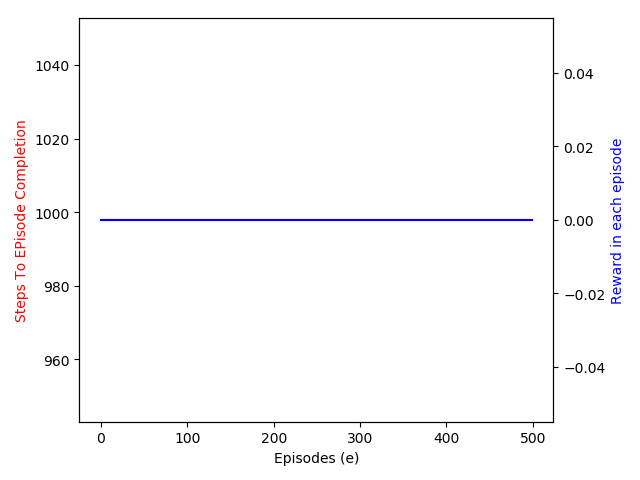
\includegraphics[width=10cm,height=10cm,keepaspectratio]{1-29_1.png}}
\caption{Graph showing total rewards when the agent stays in S1 throughout all episodes}
\label{fig}
\end{figure}

\begin{figure}[htbp]
\centerline{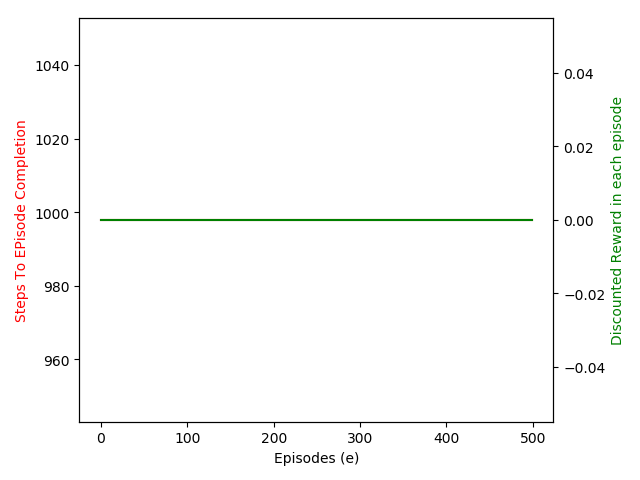
\includegraphics[width=10cm,height=10cm,keepaspectratio]{1-29_2.png}}
\caption{Graph showing discounted rewards when the agent stays in S1 throughout all episodes}
\label{fig}
\end{figure}

\begin{figure}[htbp]
\centerline{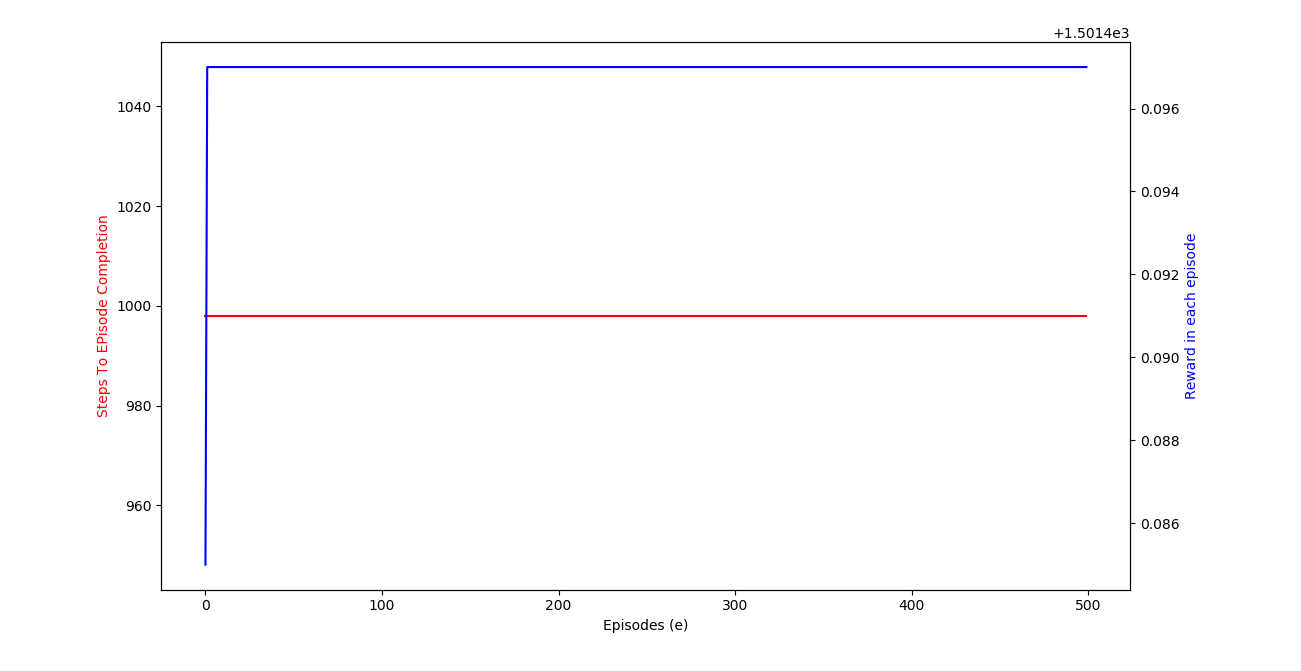
\includegraphics[width=10cm,height=10cm,keepaspectratio]{31-69_1.png}}
\caption{Graph showing total rewards when the agent stays in S2 throughout all episodes}
\label{fig}
\end{figure}

\begin{figure}[htbp]
\centerline{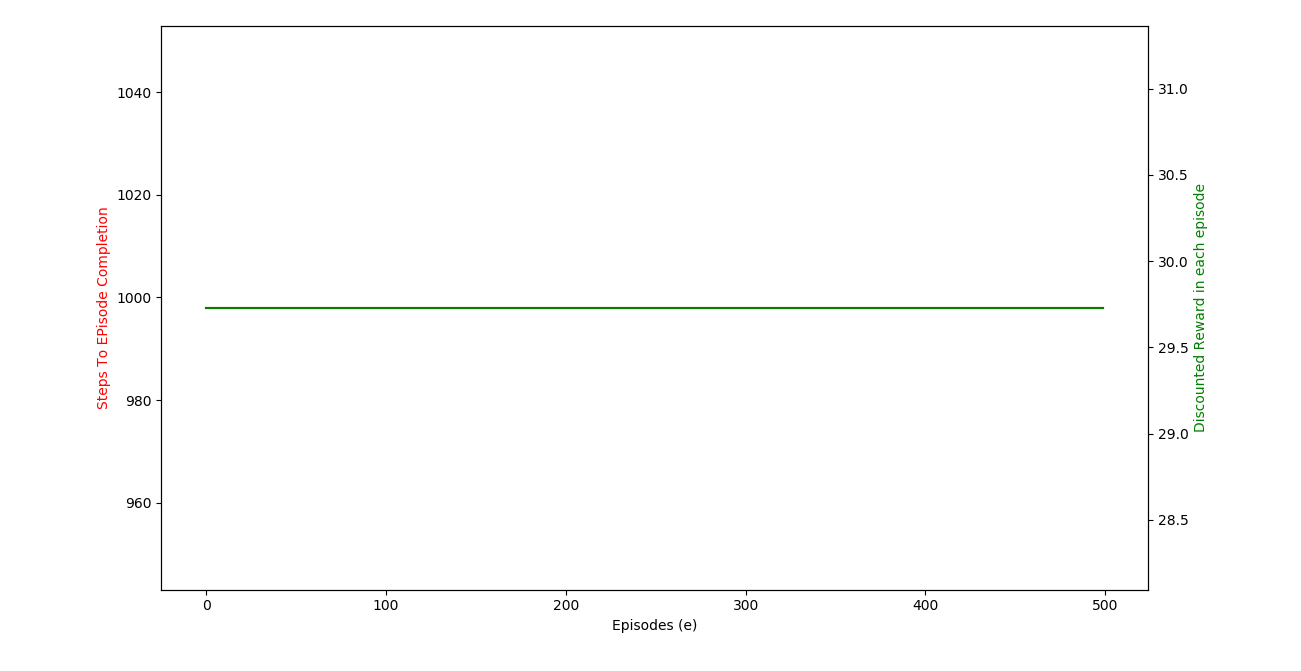
\includegraphics[width=10cm,height=10cm,keepaspectratio]{31-69_2.png}}
\caption{Graph showing discounted rewards when the agent stays in S1 throughout all episodes}
\label{fig}
\end{figure}

\begin{figure}[htbp]
\centerline{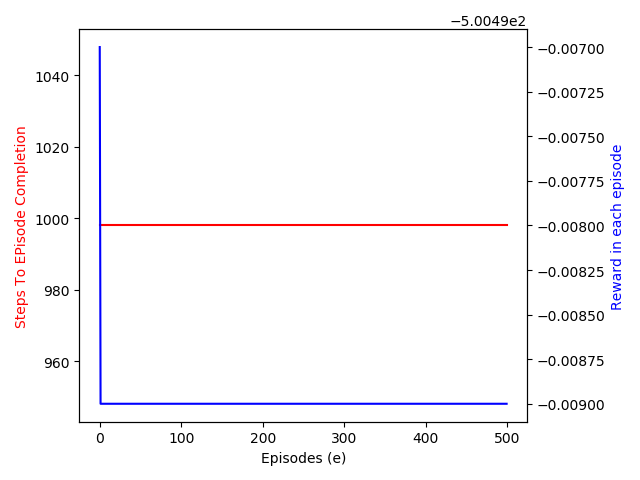
\includegraphics[width=10cm,height=10cm,keepaspectratio]{71-99_1.png}}
\caption{Graph showing total rewards when the agent stays in S3 throughout all episodes}
\label{fig}
\end{figure}

\begin{figure}[htbp]
\centerline{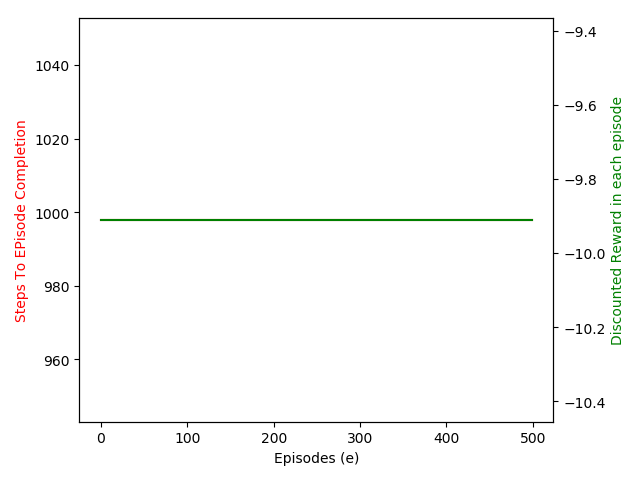
\includegraphics[width=10cm,height=10cm,keepaspectratio]{71-99_2.png}}
\caption{Graph showing discounted rewards when the agent stays in S1 throughout all episodes}
\label{fig}
\end{figure}

\begin{figure}[htbp]
\centerline{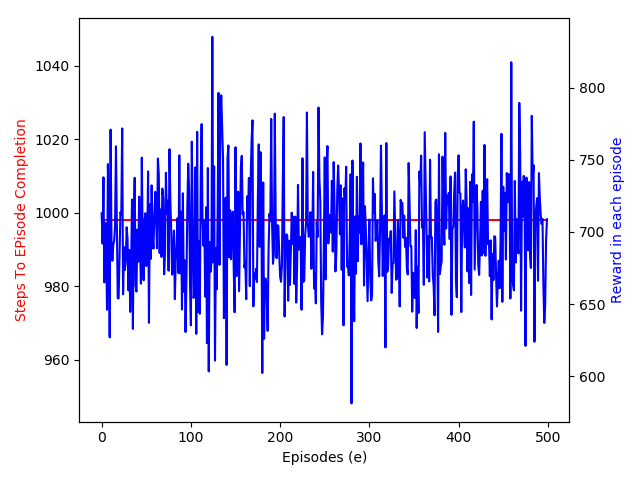
\includegraphics[width=10cm,height=10cm,keepaspectratio]{20-80_1.png}}
\caption{Graph showing total rewards when the agent goes from one state to another throughout all episodes but spends most time in S2}
\label{fig}
\end{figure}

\begin{figure}[htbp]
\centerline{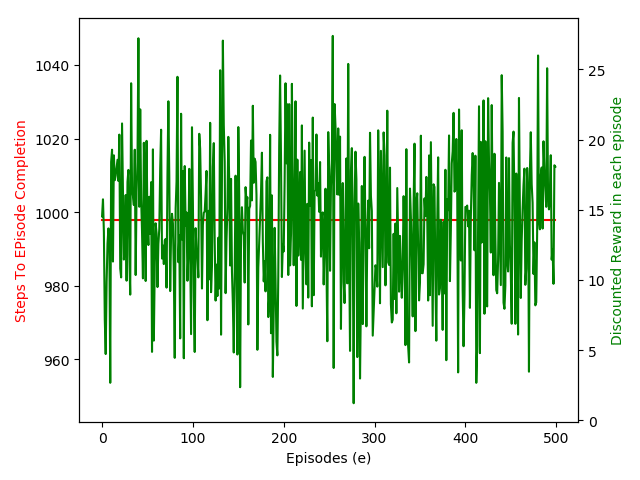
\includegraphics[width=10cm,height=10cm,keepaspectratio]{20-80_2.png}}
\caption{Graph showing discounted rewards when the agent goes from one state to another throughout all episodes but spends most time in S2}
\label{fig}
\end{figure}

Fig. 6 shows the total reward obtained when the agent stays in S1 throughout all episodes obtained for each episode (in blue) and the number of iterations (steps) in each of those episodes (in red). In this graph, the blue line overlaps the red line so it is not to be seen. From the graph, we can see that in all the episodes, the reward is same. This is because, according to Table I, a reward of 0 is given when the agent moves from S1 to itself, irrespective of whether upscaling or downscaling is performed. \\

Fig. 7 shows the discounted reward obtained when the agent stays in S1 throughout all episodes obtained for each episode (in green) and the number of iterations (steps) in each of those episodes (in red). In this graph, the blue line overlaps the red line so it is not to be seen. From the graph, we can see that in all the episodes, the discounted reward is the same. This is because, according to Table I, a reward of 0 is given when the agent moves from S1 to itself and by multiplying the discount factor with 0, the result will not change. \\

Fig. 8 shows the total reward obtained when the agent stays in S2 throughout all episodes obtained for each episode (in blue) and the number of iterations (steps) in each of those episodes (in red). From the graph, we can see that in all the episodes, the reward is the same i.e, 1500. This is because, according to Table I, a reward of +3 is given when the agent moves from S2 to itself, irrespective of whether upscaling or downscaling is performed. \\

Fig. 9 shows the discounted reward obtained when the agent stays in S2 throughout all episodes obtained for each episode (in green) and the number of iterations (steps) in each of those episodes (in red). From the graph, we can see that in all the episodes, the reward is the same. This is because, according to Table I, a reward of +3 is given when the agent moves from S2 to itself, irrespective of whether upscaling or downscaling is performed. When we multiply the total reward with the discounting factor, we get a constant value. \\

Fig. 10 shows the total reward obtained when the agent stays in S3 throughout all episodes obtained for each episode (in blue) and the number of iterations (steps) in each of those episodes (in red). From the graph, we can see that in all the episodes, the reward is the same i.e, -500. This is because, according to Table I, a reward of -1 is given when the agent moves from S3 to itself, irrespective of whether upscaling or downscaling is performed. \\

Fig. 11 shows the total reward obtained when the agent stays in S3 throughout all episodes obtained for each episode (in green) and the number of iterations (steps) in each of those episodes (in red). From the graph, we can see that in all the episodes, the reward is the same i.e, -500. This is because, according to Table I, a reward of -1 is given when the agent moves from S3 to itself, irrespective of whether upscaling or downscaling is performed. When we multiply the total reward with the discounting factor, we get a constant value. \\

Fig. 12 shows the total reward obtained when the agent goes to different episodes throughout all episodes, with a favouring to S2 though. S2 was favoured to show that the graph is not entirely random and is dense in the middle, which is close to real life situations. The total reward obtained for each episode (in blue) and the number of iterations (steps) in each of those episodes (in red) is presented in the graph. From the graph, we can see that in all the episodes, the reward is different, indicating that the rewards mechanism did work even when the agent moved from one state to another. \\

Fig. 13 shows the discounted reward obtained when the agent goes to different episodes throughout all episodes, with a favouring to S2 though. As explained above, S2 was favoured to show that the graph is not entirely random and is dense in the middle, which is close to real life situations. The total reward obtained for each episode (in green) and the number of iterations (steps) in each of those episodes (in red) is presented in the graph. From the graph, we can see that in all the episodes, the discounted reward is different as well, indicating that the discounting rewards mechanism did work even when the agent moved from one state to another. \\

From these graphs, it is clear that the agent was correctly rewarded as per the proposed rewarding method in Table I. 

 \section*{Conclusion and Future Work}

In this paper, we have worked on an LSTM predictor for predicting parameter values. From our experiments with the LSTM predictor and the RNN predictor, we can conclude that the LSTM predictor is a better choice as the RNN predictor is taking more time to converge to a value. 

We have also worked on an autoscaling algorithm using Double DQN. It was able to solve the problem as it used two networks, namely a Deep network and Target network, which help us to check the decisions made by the network using the target network and add that decision to the policy. This will help us to reduce the overestimations and get better Q-values. In the future, we will simulate the algorithm in the Kubernetes autoscaler which will help us decide the optimal values for constants like learning rate, discounting factor, epsilon decay rate other hyperparameters and better reward functions. 

\begin{thebibliography}{00}
\bibitem{b1} B. Magableh, M. Almiani, “Deep Q Learning for Self-Adaptive Distributed Microservices Architecture” (in press). IEEE Access, 2019.

\bibitem{b2} B. Magableh, “A Deep Recurrent Q Network towards Self-adapting Distributed Microservices architecture”, CoRR, cs.SE, arXiv:1901.04011, [preprint in press article accepted Jan. 2019,] doi.org/10.21427/c4v9-an45.

\bibitem{b3} S. M. R. Nouri, H. Li, S. Venugopal, W. Guo, M. He, W. Tian, "Autonomic decentralized elasticity based on a reinforcement learning controller for cloud applications", Future Gener. Comput. Syst., vol. 94, pp. 765-780, May 2019.

\bibitem{b4} F. Rossi, "Self-Management of Containers Deployment in Decentralized Environments," 2019 IEEE World Congress on Services (SERVICES), Milan, Italy, 2019, pp. 315-318.

\bibitem{b5} F. Rossi, M. Nardelli and V. Cardellini, "Horizontal and Vertical Scaling of Container-Based Applications Using Reinforcement Learning," 2019 IEEE 12th International Conference on Cloud Computing (CLOUD), Milan, Italy, 2019, pp. 329-338. doi: 10.1109/CLOUD.2019.00061

\bibitem{b6} G. Yu, P. Chen and Z. Zheng, "Microscaler: Automatic Scaling for Microservices with an Online Learning Approach," 2019 IEEE International Conference on Web Services (ICWS), Milan, Italy, 2019, pp. 68-75.
doi: 10.1109/ICWS.2019.00023

\bibitem{b7} M. Young, The Technical Writer's Handbook. Mill Valley, CA: University Science, 1989.

\bibitem{b8} S. Nanda, T.J. Hacker, “RACC: resource-aware container consolidation using a deep learning approach”, In Proc. First Workshop on Machine Learning Computing System— MLCS18, 2019, pp. 1–5.
\bibitem{b9} B. Tozer, T. Mazzuchi and S. Sarkani, "Optimizing Attack Surface and Configuration Diversity Using Multi-objective Reinforcement Learning," 2015 IEEE 14th International Conference on Machine Learning and Applications (ICMLA), Miami, FL, 2015, pp. 144-149.
\bibitem{b10} S. Iannucci, O. D. Barba, V. Cardellini, and I. Banicescu, "A Performance Evaluation of Deep Reinforcement Learning for Model-Based Intrusion Response," 2019 IEEE 4th International Workshops on Foundations and Applications of Self* Systems (FAS*W), Umea, Sweden, 2019, pp. 158-163.
\bibitem{b11} N. Belhaj, D. Belaïd and H. Mukhtar, "Framework for Building Self-Adaptive Component Applications Based on Reinforcement Learning," 2018 IEEE International Conference on Services Computing (SCC), San Francisco, CA, 2018, pp. 17-24. 

\bibitem{b12} Yenel, Atakan & Podolskiy, Vladimir & Gerndt, Michael. (2018). Predictive Auto Scaling Scheduling Application. 
\bibitem{b13} Podolskiy, Vladimir & Jindal, Anshul & Ramirez, Yesika & Yenel, Atakan & Ahmed, Saifeldin & Gerndt, Michael. (2019). SCALENDAR: Predictive Autoscaling Engine for Microservice Applications in Cloud. 10.13140/RG.2.2.18399.51361. 
\bibitem{b14} A. Kwan, J. Wong, H. Jacobsen and V. Muthusamy, "HyScale: Hybrid and Network Scaling of Dockerized Microservices in Cloud Data Centres," 2019 IEEE 39th International Conference on Distributed Computing Systems (ICDCS), Dallas, TX, USA, 2019, pp. 80-90. 
\bibitem{b15} A. U. Gias, G. Casale and M. Woodside, "ATOM: Model-Driven Autoscaling for Microservices," 2019 IEEE 39th International Conference on Distributed Computing Systems (ICDCS), Dallas, TX, USA, 2019, pp. 1994-2004.
\bibitem{b16} Bauer, André & Lesch, Veronika & Versluis, Laurens & Ilyushkin, Alexey & Herbst, Nikolas & Kounev, Samuel. (2019). Chamulteon: Coordinated Auto-Scaling of Micro-Services. 10.1109/ICDCS.2019.00199. 
\bibitem{b17} Song, B., Yu, Y., Zhou, Y. et al. J Supercomput (2018) 74: 6554. https://doi.org/10.1007/s11227-017-2044-4

\bibitem{b18} Jitendra Kumar, Ashutosh Kumar Singh, “Future Generation Computer Systems”Volume 81, April 2018, Pages 41-52

\bibitem{b19} Adel Nadjaran Toosi,Jungmin Son,Qinghua Chi,Rajkumar Buyya (2019). “ElasticSFC: Auto-scaling techniques for elastic service function chaining in network functions virtualization-based clouds” https://doi.org/10.1016/j.jss.2019.02.052
\bibitem{b20} Y. Li, L. T. X. Phan and B. T. Loo, "Network functions virtualization with soft real-time guarantees," IEEE INFOCOM 2016 - The 35th Annual IEEE International Conference on Computer Communications, San Francisco, CA, 2016, pp. 1-9.
\bibitem{b21} Volume 209, 12 October 2016, Pages 67-74. Hyun-Woo Kim,Young-Sik Jeong “Efficient auto-scaling scheme for rapid storage service using many-core of desktop storage virtualization based on IoT”
\bibitem{b22} J. Hadley, U. Roedig and Y. Elkhatib, "Using context switches for VM scaling," 2016 IEEE 35th International Performance Computing and Communications Conference (IPCCC), Las Vegas, NV, 2016, pp. 1-2.
\bibitem{b23} Y. Guo, A. Stolyar and A. Walid, "Online VM Auto-Scaling Algorithms for Application Hosting in a Cloud," in IEEE Transactions on Cloud Computing.
\bibitem{b24} G. Huang et al., "Auto scaling virtual machines for web applications with queueing theory," 2016 3rd International Conference on Systems and Informatics (ICSAI), Shanghai, 2016, pp. 433-438.
\end{thebibliography}
\vspace{12pt}

\end{document}

